\documentclass{usc-cs}
%%%%%%%%%%%%%%%%%%%%%%%%导言区%%%%%%%%%%%%%%%%%%%%%%%%%
\RequirePackage{array}
\RequirePackage{booktabs}
\RequirePackage{graphicx}
% 使用随机文本
\RequirePackage{lipsum}
% 用于调整目录行距
\RequirePackage{setspace}


% 版面设置
\RequirePackage{geometry}
\geometry{left=3.17cm,right=2.4cm,top=2.54cm,bottom=2.54cm}

% 页眉页脚
\RequirePackage{lastpage}
\RequirePackage{fancyhdr}
\pagestyle{fancy}
\lhead{}
\chead{\songti \zihao{-5}南华大学计算机学院毕业设计}
\rhead{}
\lfoot{}
\cfoot{第\thepage 页\quad 共\pageref{LastPage}页}
\rfoot{}

% 字体字号
%\renewcommand{\normalsize}{\fontsize{10pt}{\baselineskip}\selectfont}
\fontsize{12pt}{18pt}\selectfont

% 段落样式
% 首行缩进
\setlength{\parindent}{2em}
% 段落间距
% \setlength{\parskip}{0.5\baselineskip}
\setlength{\parskip}{0em}
% 设置行间距1.5倍
\setlength{\baselineskip}{1.5\baselineskip}
% \linespread{1.3}\selectfont

% 脚注设置
\renewcommand{\thefigure}{\thesection .\arabic{figure}}
\usepackage[labelsep=space]{caption}
% 使用texbib管理参考文献
\RequirePackage{cite}

% 绘图
\RequirePackage{palatino}
\RequirePackage{tikz}
\usetikzlibrary{shapes.geometric, arrows}

% 流程图定义基本形状
\tikzstyle{Node} = [rectangle, rounded corners, minimum width = 2cm, minimum height=1cm,text centered, draw = black, fill = blue!40]
\tikzstyle{arrow} = [->,>=stealth]

% 代码格式
\usepackage{listings}
\usepackage{caption}

\lstset{
	language=Python,
	basicstyle=\small\ttfamily,
	numbers=left,
	numbersep=5pt,
	xleftmargin=20pt,
	frame=tb,
	framexleftmargin=20pt
}

% 公式
\RequirePackage{amsmath}
% 表格
\RequirePackage{booktabs}
% 书签隐蔽红色框 
\usepackage[bookmarks=true]{hyperref}
\hypersetup{hidelinks}
% 书签间距
\usepackage{tocloft}
\setlength{\cftbeforesecskip}{0pt}

% 公式编号与章节关联
\numberwithin{equation}{section}






% 毕设封面
\newcommand{\cover}
{
	% 设置本页为空白
\thispagestyle{empty}

\begin{table}[ht]
	\centering
	\begin{tabular}{p{3cm}p{3cm}p{3cm}p{3cm}} 
	\multicolumn{4}{c}{
\includegraphics[width=6cm,height=6cm]{./Pictures/usc.png}}\\
	
	\specialrule{0em}{10pt}{10pt}
	\multicolumn{4}{c}{\zihao{1} \songti 计算机科学与技术学院}\\
	
	\specialrule{0em}{10pt}{10pt} 
	\multicolumn{4}{c}{\zihao{2} \kaishu 毕业设计}\\
	
	\specialrule{0em}{10pt}{5pt} 
	\songti \zihao{3}论文题目 &  \multicolumn{3}{c}{\songti \zihao{3}基于SSD网络模型的房屋瓦片损害检测}\\
	\cline{2-4} \\
	\specialrule{0em}{10pt}{5pt}
	\cline{2-4}
	
	\specialrule{0em}{10pt}{10pt} 
	\songti \zihao{3}学校导师 & \songti \zihao{3}刘立 & \songti \zihao{3}职称 & \songti \zihao{3}教授\\
	\cline{2-2}\cline{4-4}
	
	\specialrule{0em}{10pt}{10pt} 
	\songti \zihao{3}企业导师 & \songti \zihao{3} & \songti \zihao{3}职称 & \songti 	\zihao{3}\\
	\cline{2-2}\cline{4-4}
	
	\specialrule{0em}{10pt}{10pt} 
	\songti \zihao{3}
	学生姓名& \songti \zihao{3}李开运 & \songti \zihao{3}学号 & \songti \zihao{3}20144330106\\
	\cline{2-2}\cline{4-4}	
	
	\specialrule{0em}{10pt}{10pt} 
	\songti \zihao{3}
	专业班级 & \songti \zihao{3}物联网 & \songti \zihao{3}班级 & \songti \zihao{3}14级01班\\
	\cline{2-2}\cline{4-4}
	
	\specialrule{0em}{10pt}{10pt} 
	\songti \zihao{3}系主任 & \songti \zihao{3}毛宇 & \songti \zihao{3}院长 & \songti \zihao{3}刘振宇\\
	\cline{2-2}\cline{4-4}
	
	\specialrule{0em}{10pt}{10pt}		
	\songti \zihao{3}起止时间 &  \multicolumn{3}{c}{\songti \zihao{3}2017年6月5日至2018年5月22日}\\
	\cline{2-4}
	
	\specialrule{0em}{15pt}{10pt}
	\multicolumn{4}{c}{\zihao{3} \songti 2018年3月8日}\\

	\end{tabular}		
\end{table}
\newpage

}

% 重定义行间公式格式环境 
\newenvironment{uscequation}
{
	\begin{equation}
	\setlength{\abovedisplayskip}{1pt} 		
	\setlength{\belowdisplayskip}{1pt}
}
{
	\end{equation}
}

\newenvironment{uscfigure}
{
	\par
	\begin{figure}[htbp]
	\centering	
}
{	
	\end{figure}
}


\renewcommand*\thelstnumber{\arabic{lstnumber}:}

\DeclareCaptionFormat{mylst}{\hrule#1#2#3}
\captionsetup[lstlisting]{format=mylst,labelfont=bf,singlelinecheck=off,labelsep=space}



%%%%%%%%%%%%%%%%%%%%%%%%正文区%%%%%%%%%%%%%%%%%%%%%%%%%
\begin{document}
	% cover
	%\cover
	\begin{center}
	\begin{spacing}{1.5} 
		\tableofcontents
		\thispagestyle{empty}
		\pagestyle{empty} 
		\newpage
	\end{spacing}
	\end{center}
	\newpage
	\begin{uscabstract}
近年来,自然灾害的频发导致美国房屋理赔行业急需一套无损害、低成本的对房屋瓦片损害的检测方案。随着商用无人机的发展和基于深度学习的各类检测算法的出现,使得通过无人机代替工作人员进行房屋瓦片检测成为现实。本研究通过比较近年来主要的目标检测算法,考虑到瓦片的特征,采用基于SSD: Single Shot MultiBox Detector\cite{ssd}改进算法进行瓦片损害检测,实验结果满足了保险行业的要求。且检测精度达到了$65\%$mAP,检测速度达到了80fps。
\end{uscabstract}
\begin{usckeywords}
目标检测,深度学习,SSD
\end{usckeywords}

	\section*{House tile damage detection based on SSD network model}
\addcontentsline{toc}{section}{Abstract}


	\section{绪论}
% 一些关于序号的设置
\setcounter{figure}{0}

\subsection{课题背景及研究意义}\
\subsubsection{研究背景}
\textbf{自然灾害频发:}根据今日美国报道,美国国家海洋和大气管理局(NOAA)周一宣布,由于三次强大的冰雹,使2017年成为美国遭受冰雹灾害最为严重的年份之一。冰雹灾害让美国遭受了超过3000亿美元的损失。\footnote{美国中文网,2018-1-8}

\textbf{无人机的商用:}从钮扣大小的微型飞行器到可用于执行特殊任务的商用无人机,目前进入市面上的无人机种类和数量都在快速增加。较小的最低10美元就可以买到。消费类无人机的用途主要是拍摄和娱乐,那些可以执行特定任务的无人机则开始用于商业用途。

\textbf{机器视觉的发展:}近年来深度学习发展迅猛,由于谷歌的AlphaGo而轰动一时,深度学习目前还处于发展阶段,理论方面、实践方面都还有许多问题待解决,不过由于我们处在了一个“大数据”时代,以及丰富的计算资源,大大缩短了新模型、新理论的验证周期。人工智能时代的开启必然会很大程度的从人们生活的方方面面改变这个世界。

\subsubsection{研究意义}
针对传统的房屋瓦片检测方法存在着操作复杂、耗时、高危和具有破坏性等缺点,本项研究尝试利用计算机视觉技术对瓦片进行快速无损检测。本文提出了一种利用基于SSD(Single Shot MultiBox Detector)\cite{ssd}改进算法进行瓦片损害检测的方案,为房屋检测行业提供利用机器视觉处理传统检测问题的高效手段。其意义有三:

\textbf{1、无损检测:}传统的房屋瓦片损害检测工作,需要工作人员爬上房屋拍照,将照片带回工作室进行损害鉴定,这种操作无疑会对瓦片带来人为的破坏;与此同时,工作人员因操作不当受伤甚至致死的报道也时有发生 ,本项研究利用无人机替代工作人员的拍照工作,利用无人机的图像处理模块,实时进行损害的检测,将结果和图片一并送到系统中进行信息的汇总和检测报告的生成。做到的对瓦片和对工作人员的两个“无损”。

\textbf{2、缩短检测周期:}在美国,遇到自然灾害致使房屋受损后,参保的家庭会联系保险公司进行理赔,按照现在的处理水平,一栋房屋平均会耗时7个星期,对于偏远的地方会更久。采用无人机对受损房屋瓦片进行检测会将这个时长缩短到1个星期。大大节约了成本。同时实验也表明有更好的检测效果。

\textbf{3、节约人力成本:}经融危机和通货膨胀造成了人力成本的极大提高。传统的损害检测十分依赖工作人员的经验,所以人力成本一直居高不下,采用搭载了检测算法的无人机进行检测,摆脱了对工作人员经验的依赖,将成本从100美元降到了10美元。
\subsection{研究现状及发展难点}
本文主要是利用SSD改进算法对房屋瓦片损害进行检测,涉及到目标检测系列算法,对于此系列算法的研究是深度学习方向的研究热点。简单的说,目标检测算法是对物体进行定位+分类。目标检测算法与定位算法、分类算法相比,重要的区别是对图片中的对象既要定位又要判断其类别。且对象检测的输出长度是可变的,因为检测到的对象的数量是不定的。

\subsubsection{研究现状}
在深度学习正式介入之前,传统的“目标检测”方法都是区域选择、提取特征、分类回归三部曲\cite{hkq},这样就有两个难以解决且至关重要的问题;其一是区域选择的策略效果差、时间复杂度高;其二是手工提取的特征鲁棒性较差。大数据时代来临后,“目标检测”算法大家族主要划分为两大派系。

基于”Proposal + Classification”的Object Detection的方法,RCNN系列(R-CNN\cite{rcnn}、SPPnet\cite{sppnet}、Fast R-CNN\cite{fastrcnn}以及Faster R-CNN\cite{fasterrcnn})取得了非常好的效果,因为这一类方法先预先回归一次边框,然后再进行骨干网络训练,所以精度要高,这类方法被称为“Two Stage”的方法。但也正是由于此,这类方法在速度方面还有待改进。由此,YOLO\cite{yolo}应运而生,YOLO系列只做了一次边框回归和打分,所以相比于RCNN系列被称为“One Stage”的方法,这类方法的最大特点就是速度快。但是YOLO虽然能达到实时的效果,但是由于只做了一次边框回归并打分,这类方法导致了小目标训练非常不充分,对于小目标的检测效果非常的差。简而言之,YOLO系列对于目标的尺度比较敏感,而且对于尺度变化较大的物体泛化能力比较差。

针对YOLO和Faster R-CNN的各自不足与优势,WeiLiu等人提出了Single Shot MultiBox Detector,简称为SSD。SSD整个网络采取了“One Stage”的思想,以此提高检测速度。并且网络中融入了Faster R-CNN\cite{fasterrcnn}中的anchors思想,并且做了特征分层提取并依次计算边框回归和分类操作,由此可以适应多种尺度目标的训练和检测任务。SSD的出现是该时期的集大成者,向大家证明了实时高精度目标检测的可行性。

\subsubsection{发展难点}
\textbf{对象的数量可变(Variable Number of Objects)}。在训练模型时,通常需要将数据表示为固定大小的向量。但是,由于图片中对象的数量事先不知道,所以我们不知道正确的输出维度。因此需要一些后期处理,这增加了模型的复杂性。

\textbf{对象检测窗口的调整(Resizing)}。另一个巨大的挑战是各种可能的对象大小,即在进行分类时,既希望占图片大部分的对象进行分类,又想要找到一些可能只有几个像素、或者是原始图像一小部分的小对象。使用不同尺寸的滑动窗口可以解决这个问题,但效率很低。

\textbf{建模}。第三个挑战是同时解决两个问题——定位和分类如何用一个简单的模型解决这两种截然不同的需求。

\subsection{研究内容及章节安排}
第一章:绪论。本章概要阐述本文主要内容,及研究背景及意义。

第二章:目标检测相关算法。本章按照两条主线系统讲解国内外对于目标检测算法的研究。

第三章:瓦片损害检测算法设计。通过第二章的综述,我们对SSD算法进行了两点改进:

1、Loss函数
2、Soft-NMS

第四章:瓦片损害检测算法实现。本章展示具体的算法实现

第五章:实验结果及分析。本章结合经典的目标检测算法与本算法进行对比,并展示该算法对于瓦片损害检测的效果 

第六章:总结及展望。

第七章:致谢。


	\section{目标检测相关算法}
% 一些关于序号的设置
\setcounter{figure}{0}

\subsection{目标检测算法概述}
目标检测是计算机视觉领域的基础问题,在2010年左右其发展就开始停滞不前了。自2013年——\textit{Rich Feature Hierarchies for Accurate Object Detection and Semantic Segmentation}\cite{rcnn}的发表,目标检测从原始的传统手工提取特征方法变成了基于卷积神经网络的特征提取,从此一发不可收拾。根着历史的潮流,本章简要地探讨“目标检测”算法的两种思想和这些思想引申出的具有代表性的算法。

“目标检测”算法大家族主要划分为两大派系,一个是以R-CNN为代表的“Two Stage”,另一个则是以YOLO为代表的"One Stage"。下面分别解释一下“Two Stage”和“One Stage”。

\textbf{Two Stage:}顾名思义,分两步进行目标检测:1、生成可能区域(Region Proposal) \& CNN提取特征。2、放入分类器分类并修正位置。这一流派的算法都离不开Region Proposal,即是优点也是缺点,主要代表算法就是Faster R-CNN。

\textbf{One Stage:}顾名思义,对预测的目标物体直接进行检测:直接利用回归进行目标检测,其特点简单快速,但是有损精度,主要代表算法是YOLO和SSD。

无论“Two Stage”还是“One Stage”,他们都是在同一个天平下选取一个平衡点、或者选取一个极端——要么准,要么快。"Two Stage"的天平主要倾向准,“One Stage”的天平主要倾向快。但最后大家也找到了自己的平衡,平衡点的有略微的不同。接下来将分别介绍这两个派系的算法。


\subsection{R-CNN系列}
R-CNN 其实是一个很大的家族,自从 rbg 大神发表那篇论文,子孙无数、桃李满天下。在此,我们只探讨 R-CNN 直系亲属,他们的发展顺序如下:

\vspace{10pt}
%%%%%%%%%%%%%%%%%%%%%%%%%%%将要提到glossary文档中%%%%%%%%%%%%%%%%%%%%%%%%%%%%%

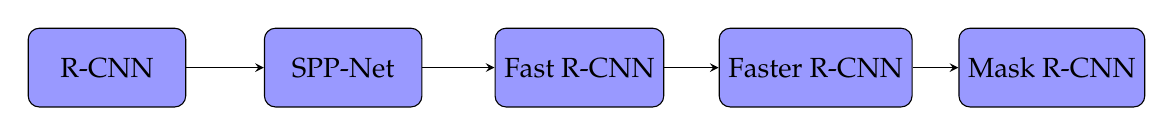
\begin{tikzpicture}[node distance=3cm]
\node (rcnn) [Node]
{R-CNN};
\node (sppnet) [Node,right of=rcnn]
{SPP-Net};
\node (fastrcnn) [Node,right of=sppnet]
{Fast R-CNN};
\node (fasterrcnn) [Node,right of=fastrcnn]
{Faster R-CNN};
\node (maskrcnn) [Node,right of=fasterrcnn]
{Mask R-CNN};
%连接具体形状
\draw [arrow] (rcnn) -- (sppnet);
\draw [arrow] (sppnet) -- (fastrcnn);
\draw [arrow] (fastrcnn) -- (fasterrcnn);
\draw [arrow] (fasterrcnn) -- (maskrcnn);
\end{tikzpicture}

他们在整个家族进化的过程中,一致暗埋了一条主线:充分榨干 feature maps 的价值。

\subsubsection{R-CNN}
这个模型,是利用卷积神经网络来做「目标检测」的开山之作,其意义深远不言而喻。
\begin{uscfigure}
	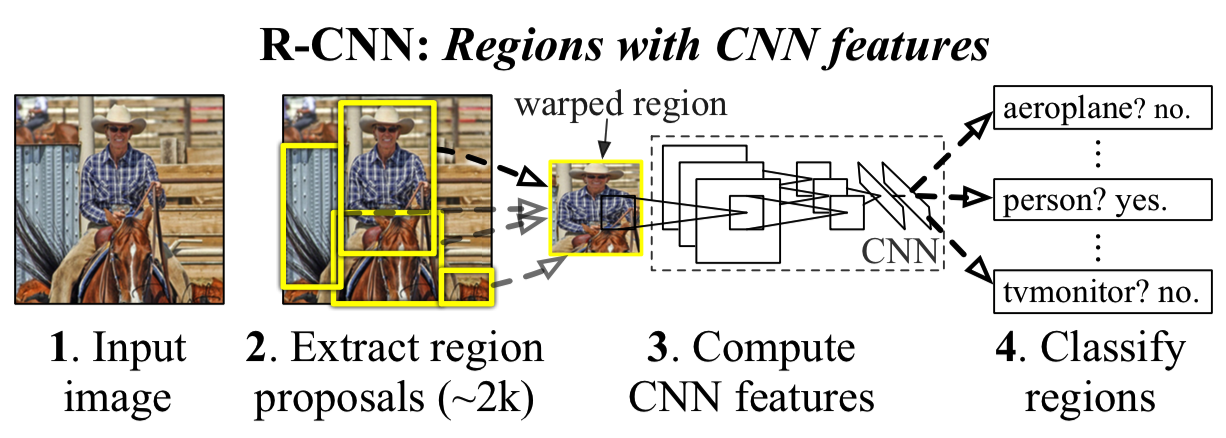
\includegraphics[width=\textwidth]{./Pictures/rcnn-regions_with_cnn_features.png}	
	\caption{RCNN}
\end{uscfigure}

\textbf{解决问题一、速度}
传统的区域选择使用滑窗,每滑一个窗口检测一次,相邻窗口信息重叠高,检测速度慢。R-CNN 使用一个启发式方法(Selective search),先生成候选区域再检测,降低信息冗余程度,从而提高检测速度。

\textbf{解决问题二、特征提取}
传统的手工提取特征鲁棒性差,限于如颜色、纹理等 低层次(Low level)的特征。使用 CNN (卷积神经网络)提取特征,可以提取更高层面的抽象特征,从而提高特征的鲁棒性。

该方法将 PASCAL VOC 上的检测率从 35.1\% 提升到 53.7 \% ,提高了好几个量级。虽然比传统方法好很多,但是从现在的眼光看,只能是初窥门径。

\subsubsection{SPP Net}
R-CNN 提出后的一年,以何恺明、任少卿为首的团队提出了 SPP Net ,这才是真正摸到了卷积神经网络的脉络。也不奇怪,毕竟这些人鼓捣出了 ResNet 残差网络,对神经网络的理解是其他人没法比的。尽管 R-CNN 效果不错,但是他还有两个硬伤:

\textbf{硬伤一、算力冗余}
先生成候选区域,再对区域进行卷积,这里有两个问题:其一是候选区域会有一定程度的重叠,对相同区域进行重复卷积;其二是每个区域进行新的卷积需要新的存储空间。何恺明等人意识到这个可以优化,于是把先生成候选区域再卷积,变成了先卷积后生成区域。“简单地”改变顺序,不仅减少存储量而且加快了训练速度。

\textbf{硬伤二、图片缩放}
无论是剪裁(Crop)还是缩放(Warp),在很大程度上会丢失图片原有的信息导致训练效果不好,如上图所示。直观的理解,把车剪裁成一个门,人看到这个门也不好判断整体是一辆车;把一座高塔缩放成一个胖胖的塔,人看到也没很大把握直接下结论。人都做不到,机器的难度就可想而知了。
\begin{uscfigure}
	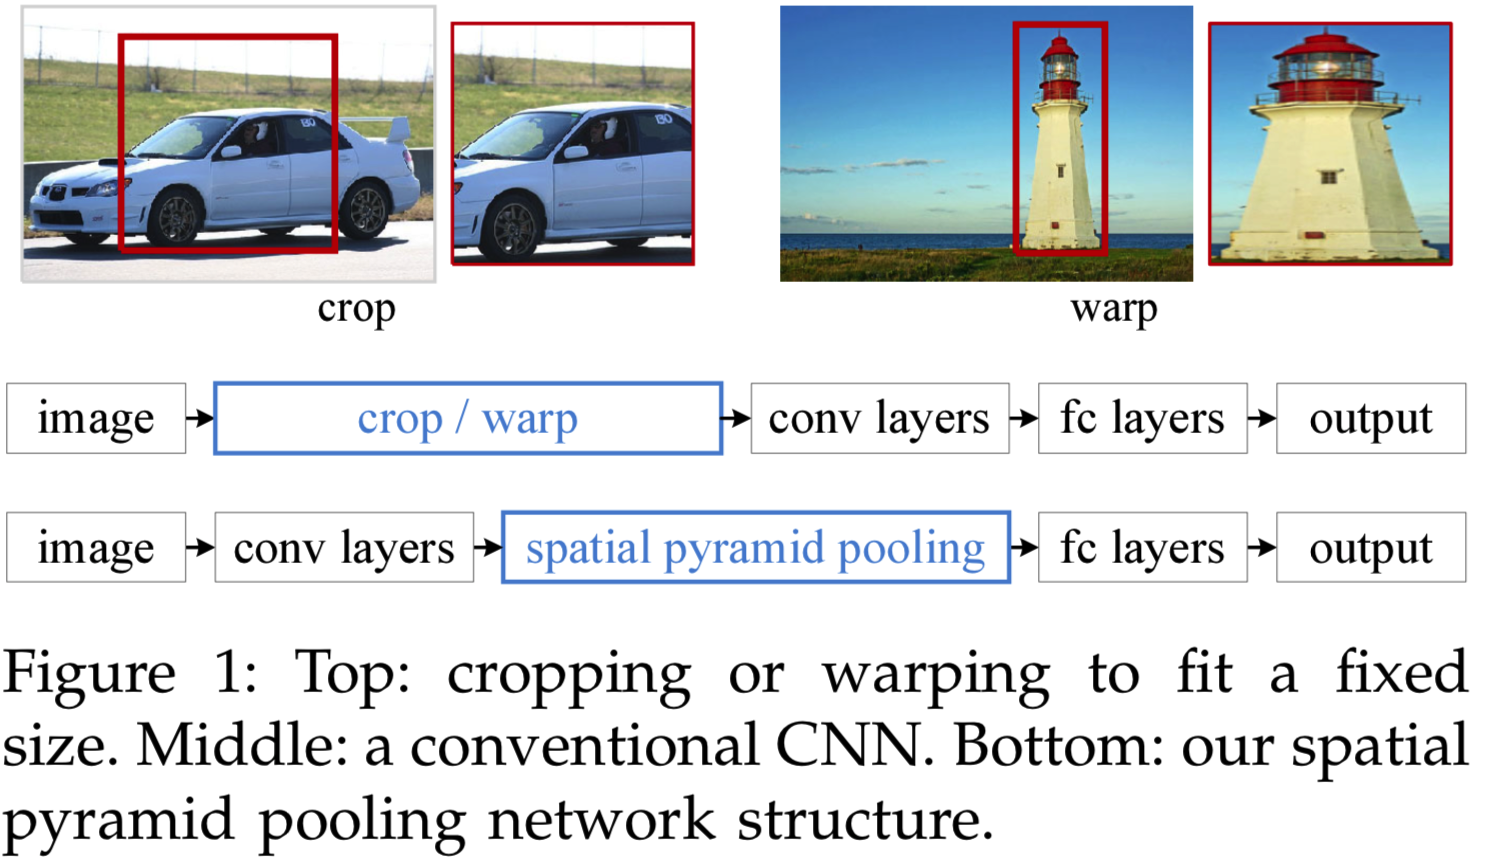
\includegraphics[width=\textwidth]{./Pictures/sppnet_crop_warp.png}	
	\caption{RCNN}
\end{uscfigure}
何恺明等人发现了这个问题,于是思索有什么办法能不对图片进行变形,将图片原汁原味地输入进去学习。最后,他们发现问题的根源是 FC Layer(全连接层)需要确定输入维度,于是他们在输入全连接层前定义一个特殊的池化层,将输入的任意尺度 feature maps 组合成特定维度的输出,这个组合可以是不同大小的拼凑,如同拼凑七巧板般。举个例子,我们要输入的维度 64∗256 ,那么我们可以这样组合 32∗256+16∗256+8∗256+8∗256 。
\begin{uscfigure}
	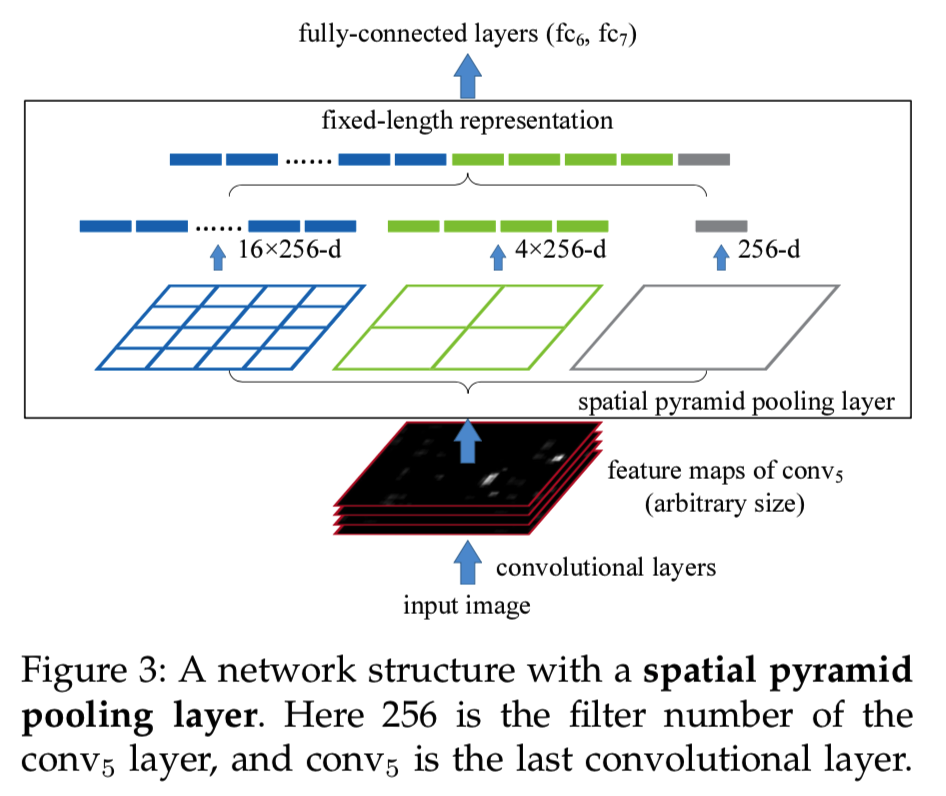
\includegraphics[width=\textwidth]{./Pictures/sppnet_pool_layer.png}	
	\caption{RCNN}
\end{uscfigure}
SPP Net 的出现是如同一道惊雷,不仅减少了计算冗余,更重要的是打破了固定尺寸输入这一束缚,让后来者享受到这一缕阳光。

\subsubsection{Fast R-CNN}
在这篇论文中,引用了 SPP Net 的工作,并且致谢其第一作者何恺明的慷慨解答。纵观全文,最大的建树就是将原来的串行结构改成并行结构
\begin{uscfigure}
	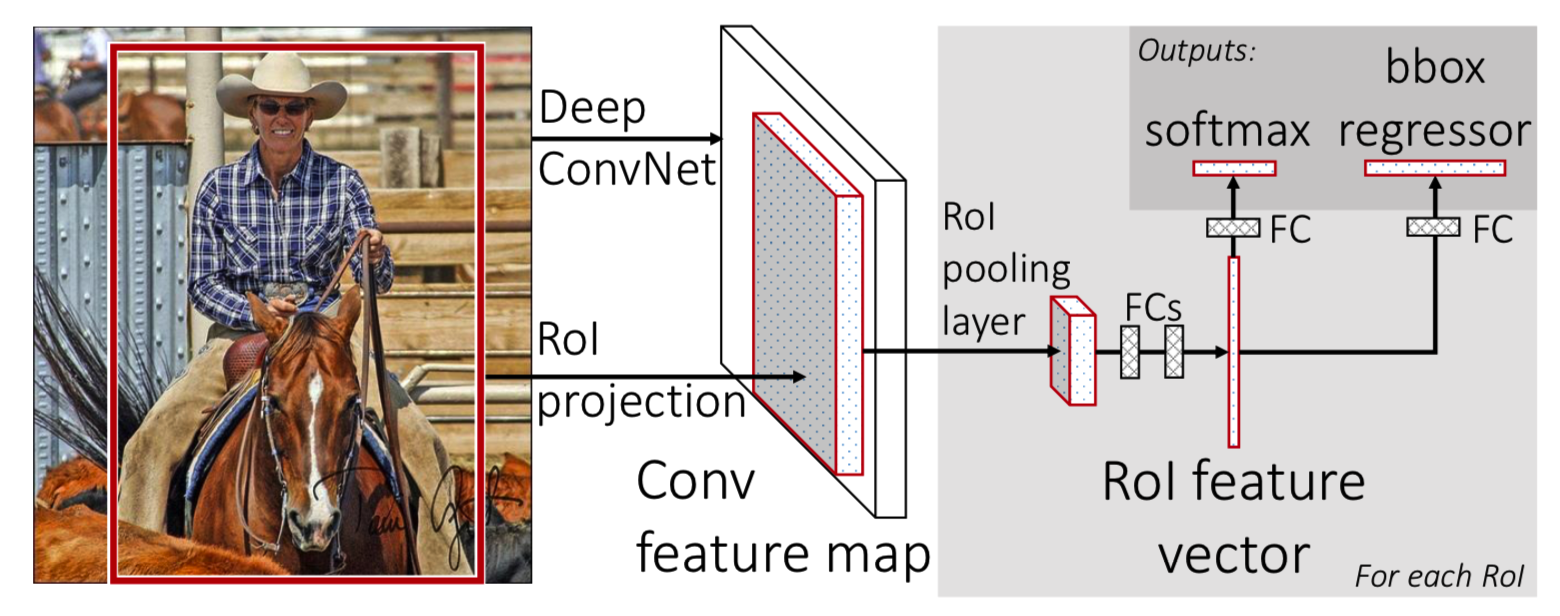
\includegraphics[width=\textwidth]{./Pictures/fast_rcnn.png}	
	\caption{RCNN}	
\end{uscfigure}
原来的 R-CNN 是先对候选框区域进行分类,判断有没有物体,如果有则对 Bounding Box 进行精修 回归。这是一个串联式的任务,那么势必没有并联的快,所以 rbg 就将原有结构改成并行——在分类的同时,对 Bbox 进行回归。这一改变将 Bbox 和 Clf 的 loss 结合起来变成一个 Loss 一起训练,并吸纳了 SPP Net 的优点,最终不仅加快了预测的速度,而且提高了精度。
\subsubsection{Faster R-CNN}
在 Faster R-CNN 前,我们生产候选区域都是用的一系列启发式算法,基于 Low Level 特征生成区域。这样就有两个问题:

第一个问题 是生成区域的靠谱程度随缘,而 两刀流 算法正是依靠生成区域的靠谱程度——生成大量无效区域则会造成算力的浪费、少生成区域则会漏检;

第二个问题 是生成候选区域的算法是在 CPU 上运行的,而我们的训练在 GPU 上面,跨结构交互必定会有损效率。

那么怎么解决这两个问题呢?于是乎,任少卿等人提出了一个 Region Proposal Networks 的概念,利用神经网络自己学习去生成候选区域。
\begin{uscfigure}
	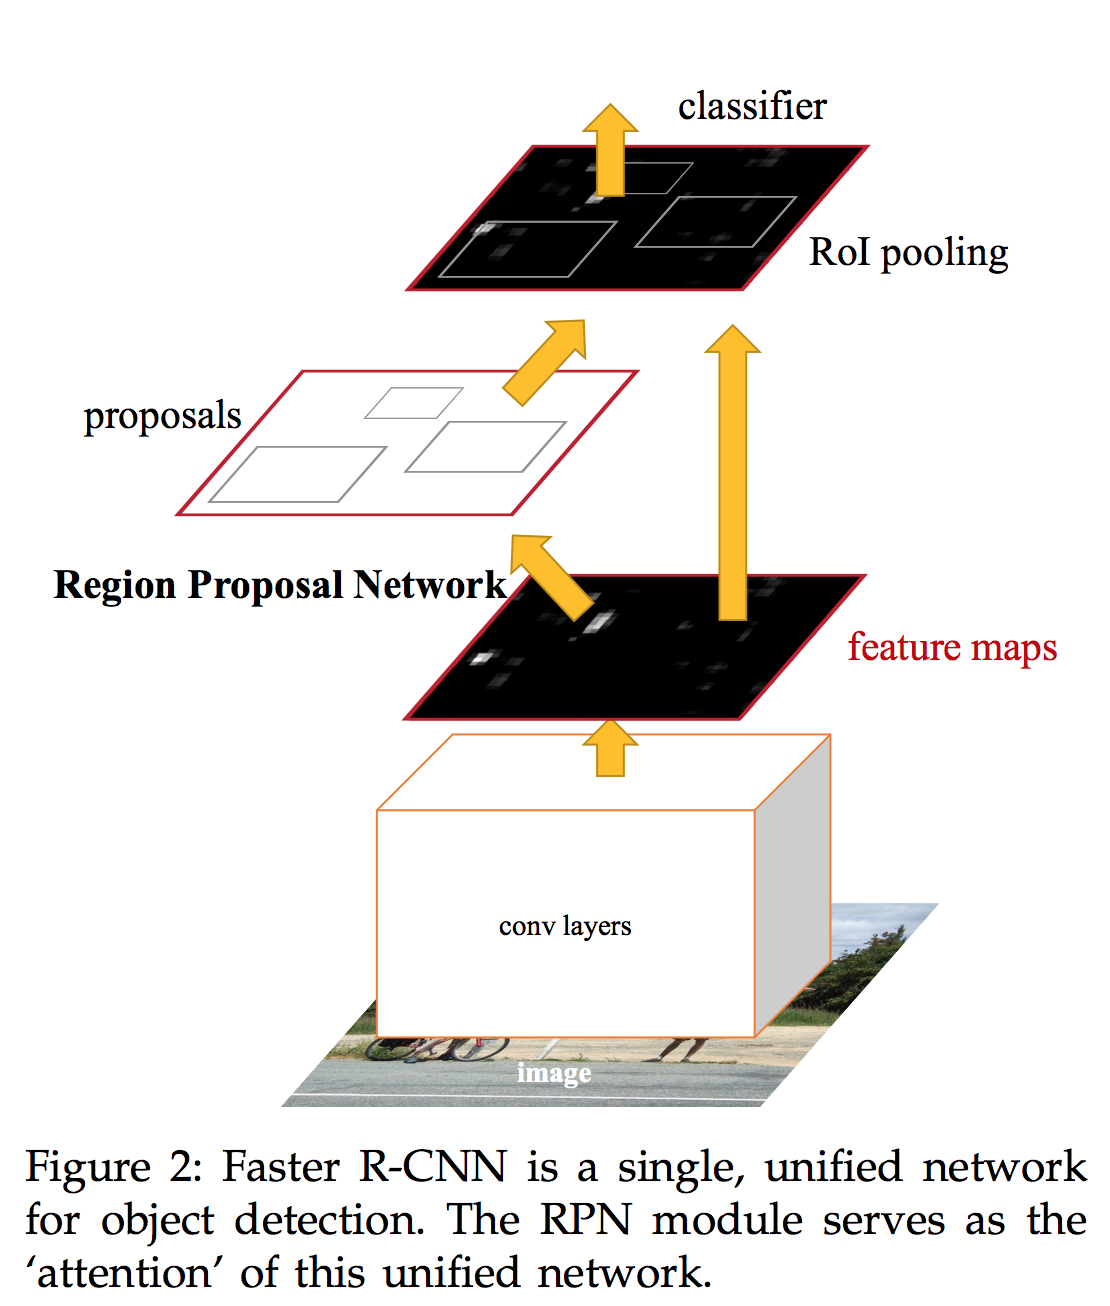
\includegraphics[width=\textwidth]{./Pictures/faster_rcnn.png}	
	\caption{RCNN}	
\end{uscfigure}
这种生成方法同时解决了上述的两个问题,神经网络可以学到更加高层、语义、抽象的特征,生成的候选区域的可靠程度大大提高;可以从上图看出 RPNs 和 RoI Pooling 共用前面的卷积神经网络——将 RPNs 嵌入原有网络,原有网络和 RPNs 一起预测,大大地减少了参数量和预测时间。
\begin{uscfigure}
	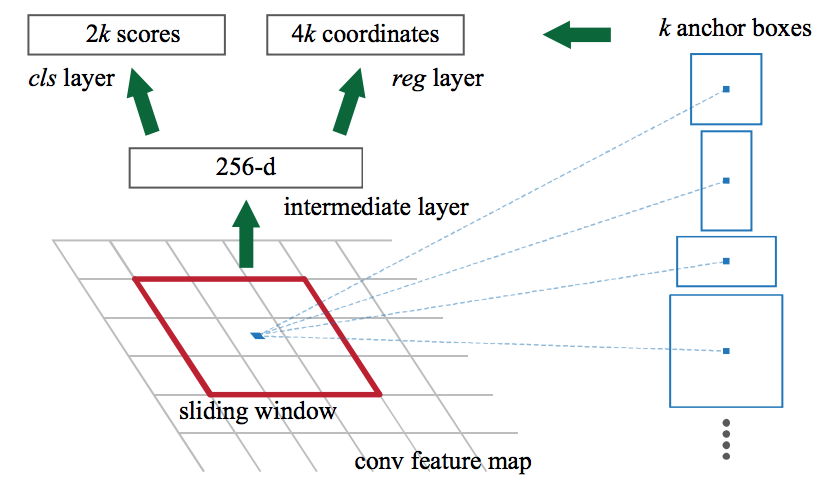
\includegraphics[width=\textwidth]{./Pictures/faster_rcnn_anchor.png}	
	\caption{RCNN}	
\end{uscfigure}
在 RPNs 中引入了 anchor 的概念,feature map 中每个滑窗位置都会生成 k 个 anchors,然后判断 anchor 覆盖的图像是前景还是背景,同时回归 Bbox 的精细位置,预测的 Bbox 更加精确。
\subsubsection{Mask R-CNN}
时隔一年,何恺明团队再次更新了 R-CNN 家族,改进 Faster R-CNN 并使用新的 backbone 和 FPN 创造出了 Mask R-CNN 。

\textbf{加一条通道}

我们纵观发展历史,发现 SPP Net 升级为 Fast R-CNN 时结合了两个 loss ,也就是说网络输入了两种信息去训练,结果精度大大提高了。何恺明他们就思考着再加一个信息输入,即图像的 Mask ,信息变多之后会不会有提升呢?于是乎 Mask R-CNN 就这样出来了,不仅可以做「目标检测」还可以同时做「语义分割」,将两个计算机视觉基本任务融入一个框架。没有使用什么 trick ,性能却有了较为明显的提升,这个升级的版本让人们不无啧啧惊叹。作者称其为 meta algorithm ,即一个基础的算法,只要需要「目标检测」或者「语义分割」都可以使用这个作为 Backbone 。



\subsection{YOLO系列}
YOLO是单阶段方法的开山之作。它将检测任务表述成一个统一的、端到端的回归问题,并且以只处理一次图片同时到位置和分类而得名。一刀流的想法就比较暴力,给定一张图像,使用回归的方式输出这个目标的边框和类别。一刀流最核心的还是利用了分类器优秀的分类效果,首先给出一个大致的范围(最开始就是全图)进行分类,然后不断迭代这个范围直到一个精细的位置,
\begin{uscfigure}
	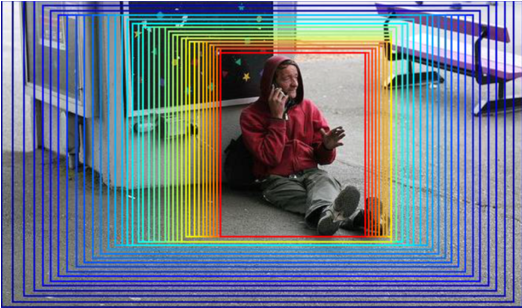
\includegraphics[width=\textwidth]{./Pictures/od_regressor.png}	
	\caption{RCNN}	
\end{uscfigure}
如上图从蓝色的框框到红色的框框。这就是一刀流回归的思想,这样做的优点就是快,但是会有许多漏检。

\subsubsection{YOLO}
\textbf{YOLO}就是使用回归这种做法的典型算法。首先将图片 Resize 到固定尺寸,然后通过一套卷积神经网络,最后接上 FC 直接输出结果,这就他们整个网络的基本结构。更具体地做法,是将输入图片划分成一个 SxS 的网格,每个网格负责检测网格里面的物体是啥,并输出 Bbox Info 和 置信度。这里的置信度指的是 该网格内含有什么物体 和 预测这个物体的准确度。

更具体的是如下定义:
\[
	Pr(Class_i | Object) * Pr(Object) * IOU_{pred}^{truth} = Pr(Class_i) * IOU_{pred}^{truth}
\]
这个想法其实就是一个简单的分而治之想法,将图片卷积后提取的特征图分为 SxS 块,然后利用优秀的分类模型对每一块进行分类,将每个网格处理完使用 NMS (非极大值抑制)的算法去除重叠的框,最后得到我们的结果。
\subsubsection{SSD}
YOLO 这样做的确非常快,但是问题就在于这个框有点大,就会变得粗糙——小物体就容易从这个大网中漏出去,因此对小物体的检测效果不好。

所以 SSD 就在 YOLO 的主意上添加了 Faster R-CNN 的 Anchor 概念,并融合不同卷积层的特征做出预测。

第三章将详细阐述SSD算法

\subsubsection{YOLO9000}
到了 SSD ,回归方法的目标检测应该一统天下了,但是 YOLO 的作者不服气,升级做了一个 YOLO9000 ——号称可以同时识别 9000 类物体的实时监测算法。讲道理,YOLO9000 更像是 SSD 加了一些 Trick ,而并没有什么本质上的进步:

加了 BN 层,扩大输入维度,使用了 Anchor,训练的时候数据增强…所以强是强,但没啥新意,SSD 和 YOLO9000 可以归为一类。


\subsection{本章小结}
R-CNN系列算法是一个很庞大的算法簇,Ross Girshick发表\textit{Rich Feature Hierarchies for Accurate Object Detection and Semantic Segmentation}\cite{rcnn}一文以来衍生出非常多的算法。在此,我们只介绍与R-CNN关系最亲密的算法,他们的发展顺序如图\ref{rcnn-dev}:
\begin{uscfigure}
	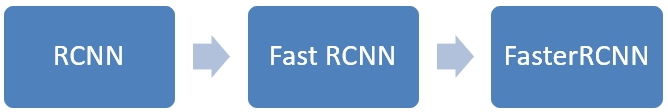
\includegraphics[width=\textwidth]{./Pictures/rcnn.jpg}	
	\caption{RCNN系列算法发展顺序}
	\label{rcnn-dev}
\end{uscfigure}

\par \noindent
他们在整个算法簇发展的过程中,更充分地利用Feature Maps的信息是系列算法发展的脉络。
\subsubsection{R-CNN}
RCNN:(Region CNN)\cite{rcnn}首次将深度学习应用到目标检测算法中。在PASCAL VOC\footnote{计算机视觉里面很大一块是在做物体的识别、检测还有分类(object recognition, detection and classification)。几乎在每一个应用领域都需要用到这三项功能,所以能否顺利的完成这三个功能,对检验一个算法的正确性和效率来说是至关重要的。所以每一个算法的设计者都会运用自己搜集到的场景图片对算法进行训练和检测,这个过程就逐渐的形成了数据集}的目标检测竞赛中,其作者Ross Girshick多次带领团队折桂。图\ref{rcnn}这个模型,“目标检测”领域内第一次结合了神经网络的结构图,其深远意义不言而喻。
\begin{uscfigure}
	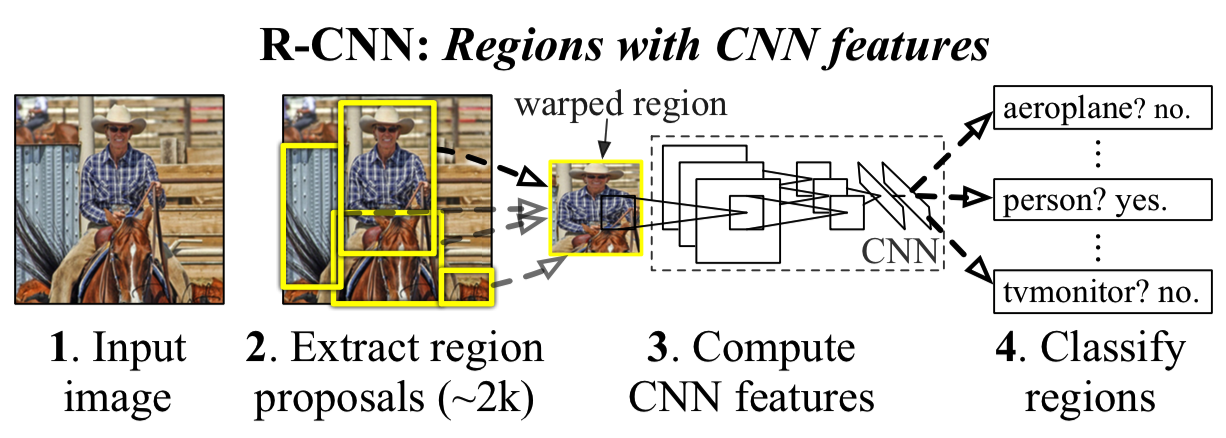
\includegraphics[width=\textwidth]{./Pictures/rcnn-regions_with_cnn_features.png}	
	\caption{RCNN算法框架}
	\label{rcnn}
\end{uscfigure}
该算法对目标检测中的两个关键问题提供了重要思路:

\textbf{解决问题一、速度。}
R-CNN使用启发式搜索方法(Selective Search\cite{ss})取代使用滑窗的区域选择算法。传统的区域选择算法,滑动一个窗口就需要检测一次,因此相邻窗口信息重叠高,导致检测速度慢。启发式搜索方法先生成候选区域再检测,大大降低了信息冗余的程度,从而检测速度得到提高。

\textbf{解决问题二、特征的鲁棒性。}
R-CNN使用卷积神经网络(CNN)提取特征取代人工设定的特征如Haar、HOG等。传统的手工提取特征鲁棒性差,特征设计复杂。仅限于低层次(Low-level)的特征如颜色、纹理等。使用CNN可以提取更高层面的抽象特征,从而提高特征的鲁棒性。

该方法将PASCAL VOC上的检测率从35.1\% 提高到53.7 \% 。

\textbf{算法流程:}

\line
\begin{itemize}
	\setlength{\itemsep}{0pt}
	\setlength{\parsep}{0pt}
	\setlength{\parskip}{0pt}
	\item[>] 一张图像生成1K至2K个候选区域;
	\item[>] 对每个候选区域,使用深度网络提取特征;
	\item[>] 特征送入每一类的SVM分类器,判别是否属于该类;
	\item[>] 使用回归器精细修正候选位置;
\end{itemize}
\line

\textbf{1、生成候选区域:}利用Selective Search\cite{ss}算法从原始图像中生成约2k-3k个候选区域。生成步骤:1、先将原始图像分割成小块区域。2、检索所有的小区域,合并最可能是属于同一个物体的两个区域。重复该操作直到整张图像中只剩下一个位置区域。3、输出所有候选的区域包括合并的区域,共同作为所谓的候选区域。

\textbf{2、提取特征:}利用2012年,Hinton在Image Net竞赛上提出的神经网络\footnote{Hinton在2012年提出的AlexNet网络}提取图像中的特征。

\textbf{3、判断类别:}对于每一类别的目标,使用线性SVM\cite{svm}分类器进行判别。输入为4096维特征向量,输出为此类别的置信度。同时原算法使用"Hard Negative Mining"\cite{hnm}方法。使正负样本的数量保持平衡。

\textbf{4、精修位置:}目标检测的结果好不好是看检测框与实际位置的重叠面积,故需要对检测的位置进行精修,以此提高检测精度。 

\subsubsection{SPP Net}
R-CNN提出后的一年,以何恺明、任少卿为首的团队发表了SPP Net:\textit{Spatial Pyramid Pooling in Deep Convolutional Networks for Visual Recognition}\cite{sppnet} ,这才是真正摸到了卷积神经网络的脉络。尽管R-CNN效果不错,但是他还有两个缺点:

\textbf{缺点一、算法过程冗余。}
R-CNN算法是先生成候选区域,再对该区域进行卷积,其导致的问题有二:其一是对相同区域进行了多次卷积,因为候选区域难免会有大量交叠的区域;其二是对存储空间浪费巨大,因为每个候选区域进行卷积后都需要新的存储空间。何恺明等人针对上述两点不足,交换了生成候选区域与卷积的顺序,通过巧妙地改变,不仅减少存储量而且大幅度地提高了训练速度。

\textbf{缺点二、图片缩放、裁剪问题。}
如图\ref{sppnet}所示,对于原始图片无论是缩放(Warp)还是裁剪(Crop),都会使原始图片的信息很大程度上的丢失从而影响训练效果。从示例图中可以看出,当把小车剪裁成一个车门,人们看到这个裁剪后的图片就难以判断图片的整体目标是一辆车;把一座高塔图片进行缩放后,也会使得机器的识别难度巨大。
\begin{uscfigure}
	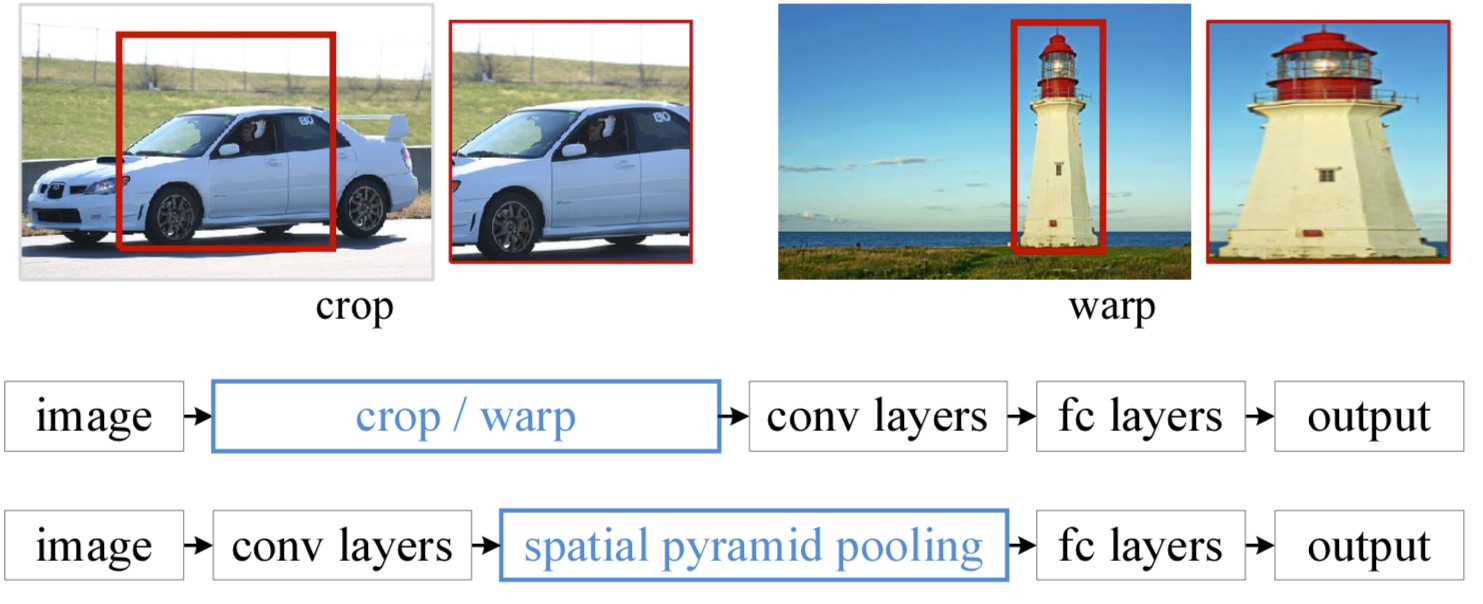
\includegraphics[width=\textwidth]{./Pictures/sppnet_crop_warp.jpg}	
	\caption{因剪裁和缩放导致视差}
	\label{sppnet}
\end{uscfigure}
问题的关键在于找到一个不对图片进行变形,且依然保留了原图整体信息的方法直接进行学习。最后,何恺明等人找到了问题的根源:全连接层(FC Layer)需要固定其输入向量维度,于是只需要定义一个特殊的池化层,使其输出的维度满足全连接层固定输入维度的要求即可。这个特殊的池化层将输入的任意尺度Feature Maps组合成特定维度的输出,如图\ref{sppnet},我们要输入的维度 $64∗256$ ,那么我们可以这样组合 $32∗256+16∗256+8∗256+8∗256$。
\begin{uscfigure}
	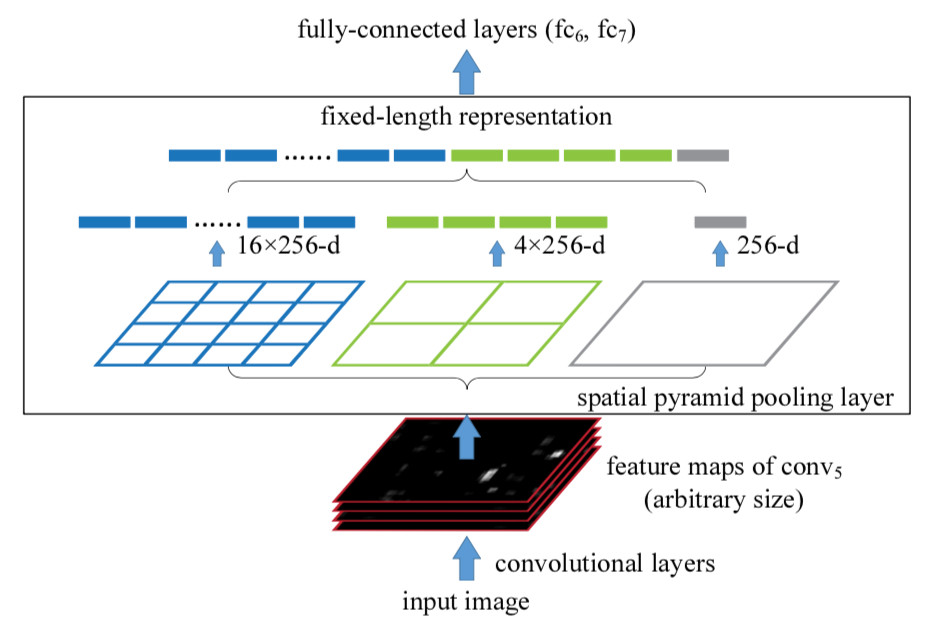
\includegraphics[width=\textwidth,]{./Pictures/sppnet_pool_layer.jpg}	
	\caption{输入维度的组合方式}
	\label{sppnet}
\end{uscfigure}
SPP Net的出现对整个目标检测及其相关领域产生了重要的影响,他不仅减少了计算冗余从而提高了检测速度,更重要的意义在于解禁了输入固定尺寸这一束缚,也因此被后面出现的算法广泛采用。本文基于的SSD算法就是更是从中受到启发。

\subsubsection{Fast R-CNN}
继2014年的RCNN之后,Ross Girshick在2015年发表了Fast RCNN\cite{fastrcnn},构思巧妙,算法流程更加紧凑,目标检测的速度也大幅提高。Fast R-CNN引用了SPP Net的贡献 。概括来说,贡献最大的地方在于用并行结构替换了原算法中的串行结构。Fast RCNN和RCNN相比,同样使用最大规模的网络,测试时间从47秒减少为0.32秒,训练时间从84小时减少为9.5小时。在PASCAL-VOC2007上的准确率,约在66\%-67\%之间。其算法框架如图\ref{fast-rcnn}
\begin{uscfigure}
	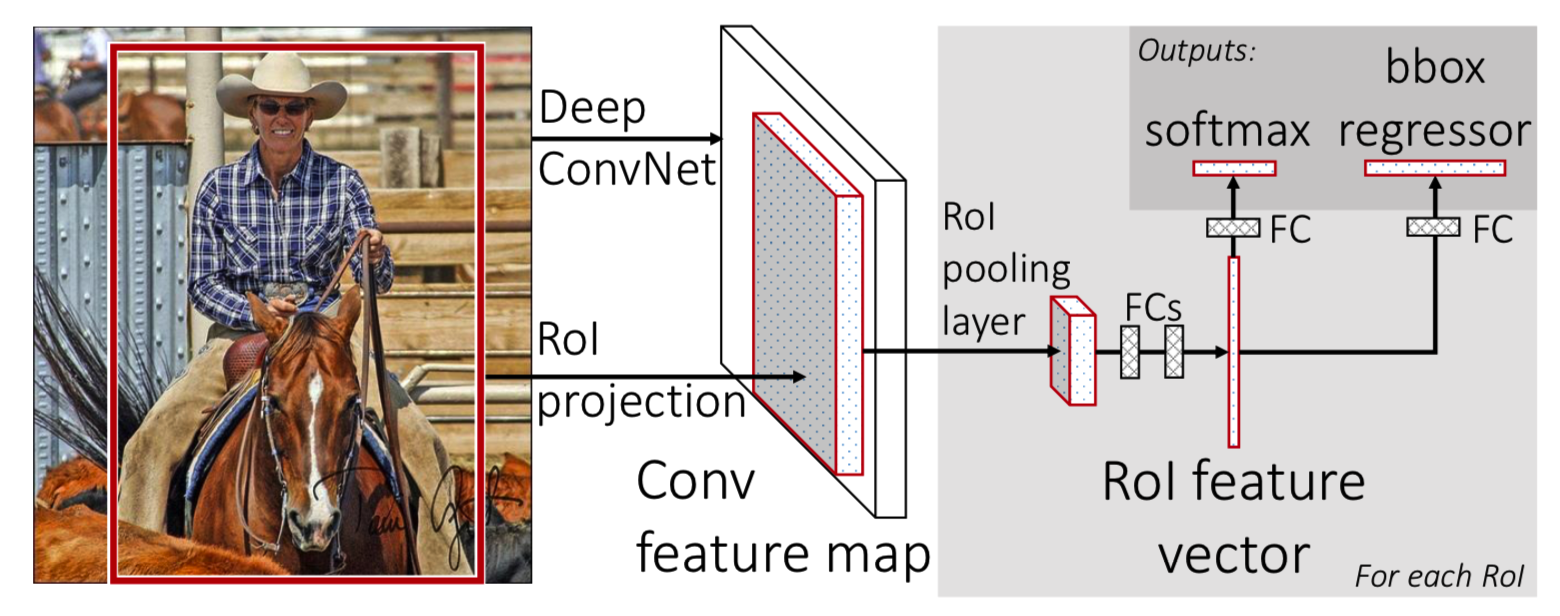
\includegraphics[width=\textwidth]{./Pictures/fast_rcnn.png}	
	\caption{Fast R-CNN算法框架}	
	\label{fast-rcnn}
\end{uscfigure}
R-CNN算法是先对候选框区域进行分类,如果检测到目标则对边界框(Bounding Box)进行精修、回归。全过程是串联的。能不能改成并联的呢?Ross Girshick将算法过程改成了并行结构——边分类,边对Bounding box进行回归。用一个Loss函数将conf-loss和loc-loss整合到了一起,同时也吸收了SPP Net算法的长处,因此其速度和精度都得到了提高。

\textbf{算法流程:}

\line
\begin{itemize}
	\setlength{\itemsep}{0pt}
	\setlength{\parsep}{0pt}
	\setlength{\parskip}{0pt}
	\item[>] 在图像中确定1000-2000个候选框 
	\item[>] 对于每个候选框内图像块,使用深度网络提取特征
	\item[>] 对候选框中提取出的特征,使用分类器判别是否属于一个特定类
	\item[>] 对于属于某一特征的候选框,用回归器进一步调整位置
\end{itemize}
\line\\
Fast RCNN算法针对RCNN算法中的三个方面进行了改进:

\textbf{第一个方面、测试时的速度慢。}由于RCNN算法中对一张图像内的候选框之间存在大量交叠部分,所以提取特征时的操作冗余,Fast R-CNN算法将整张归一化后的图像直接送入深度神经网络中。在与后面的网络邻接时,才将候选框的信息加入进来,从而共享了卷积操作,达到了提高速度的目的。

\textbf{第二个方面、训练时的速度慢。}其具体的原因同第一个方面,在训练时候,先将一张归一化后的图像送入深度神经网络中,紧接着将这幅图像上提取出的候选区域传入网络。所以避免了候选区域特征的重复计算。

\textbf{第三个方面、训练存储空间大。}RCNN算法中需要大量特征作为训练样本用来训练独立的分类器和回归器,Fast R-CNN不需要额外的存储,将类别判断和位置精修合并到一起,用一个统一的深度神经网络来实现。其网络模型如图\ref{fast-rcnn-model}

\begin{uscfigure}
	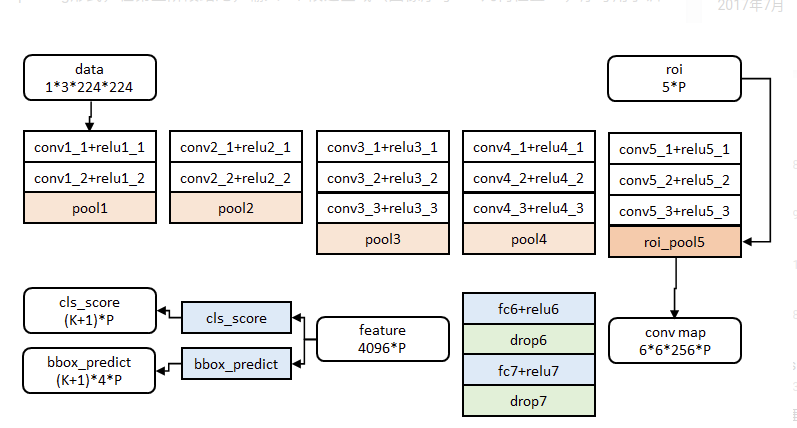
\includegraphics[width=\textwidth]{./Pictures/fast-rcnn-model.png}	
	\caption{Fast R-CNN网络模型}	
	\label{fast-rcnn-model}
\end{uscfigure}

\textbf{损失函数:}
loss\_cls评估分类损失。由其真实类别$u$对应的概率决定:
\begin{equation}
	L_{cls} = - \log p_u
\end{equation}
loss\_bbox评估检测框定位损失。由其真实类别对应的预测位置参数$t^u$和真实位置关于平移缩放$v$的因子来决定:
\begin{equation}
	L_{loc} = \sum_{i=1}^{4} g(t_i^u - v_i)
\end{equation}
	
g为Smooth L1误差,对outlier不敏感:
\begin{equation}
	g(x) = \left \{
		\begin{aligned}
		& 0.5x^2 	 & |x| < 1	\\	
		& |x| - 0.5  &otherwise
		\end{aligned}
		\right .
\end{equation}
如果分类为背景则不考虑定位代价,最后总的损失为二者加权和:
\begin{equation}
	L = \left \{
		\begin{aligned}
		& L_{cls} + \lambda L_{loc} & u\\
		& L_{cls} 					& u
		\end{aligned}
	\right .
\end{equation}
\subsubsection{Faster R-CNN}
继发表RCNN,Fast RCNN两篇力作之后,Ross Girshick等人又在2015年提出了Faster R-CNN\cite{fasterrcnn}算法。该算法在PASCAL VOC数据集上准确率为59.9\%,在简单网络目标上的检测速度达到17FPS;复杂网络目标上的检测准确率78.8\%,速度达到5FPS。在Faster R-CNN算法被提出前,所有的目标检测算法都是基于Low Level特征采用启发式搜索算法生产候选区域。这种策略存在着两个缺点:

\textbf{第一个缺点}候选区域具有不确定性。“Two Stage”系列算法为了解决这个问题生成了大量无效区域造成了大量多余的计算、可是如果减少了候选区域则又会使之漏检;

\textbf{第二个缺点}算法第一步——生成候选区域的算法是在CPU上运行的,与在GPU上训练的跨结构交互损失了算法效率。

于是乎,针对上述两个缺点,任少卿等人提出利用神经网络代替Selective Search算法自己去学习生成候选区域。将这个网络称之为RPN:Region Proposal Networks。其结构如图\ref{rpn}。
\begin{uscfigure}
	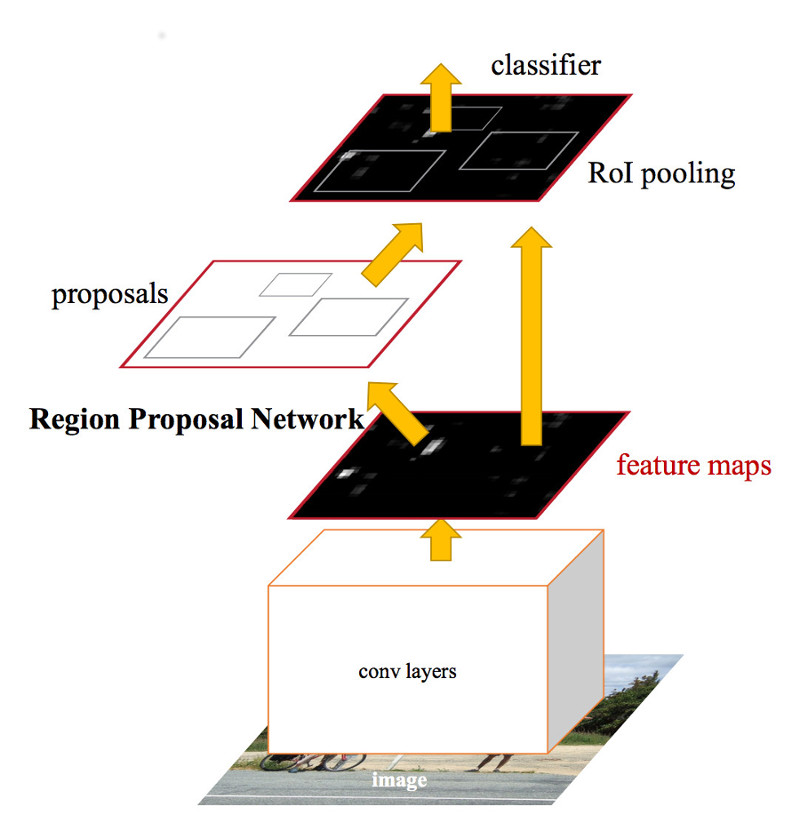
\includegraphics[width=\textwidth,height=8cm]{./Pictures/faster_rcnn.jpg}	
	\caption{Faster RCNN算法架构}	
	\label{rpn}
\end{uscfigure}
神经网络可以学到比Low Leval特征更加抽象、语义、高层的特征,同时大大提高了候选区域的可靠程度,利用RPN生成候选区域的方法一石二鸟,可以从图\ref{rpn}看出,将RPNs嵌入原有网络使RPNs和RoI Pooling层共用前面的卷积神经网络,整合原有网络和RPNs网络一起参与预测,参数量和预测时间都有在幅度的减少。值得一提的是,在RPN中引入了anchor的概念。对于Feature Map中的每个滑窗位置都会生成k个anchors,然后根据anchor与ground truth的IOU判断anchor覆盖的图像区域是前景还是背景,判断的同时回归Bounding box的精细位置。

Faster RCNN是RCNN系列算法中的集大成者,将目标检测算法的基本步骤\footnote{候选区域生成,特征提取,分类,位置精修}整合到了一个深度网络框架之内。其中所有计算共享,全部在GPU中完成,速度和精度都得到了极大的提高。

Faster RCNN始终围绕着三个问题展开:

\line
\begin{itemize}
	\setlength{\itemsep}{0pt}
	\setlength{\parsep}{0pt}
	\setlength{\parskip}{0pt}
	\item[>] 如何设计区域生成网络?
	\item[>] 如何训练区域生成网络?
	\item[>] 如何让区域生成网络和Faster RCNN网络共享特征提取网络?
\end{itemize}
\line

\textbf{区域生成网络(RPN)}

\textbf{1、特征提取:}如图\ref{rpn}灰色方框,是对原始特征提取(用任何分类模型进行提取都可)

\textbf{2、候选区域:}对于图像中的每一个位置,约定9个设定的候选窗口:三种不同比例{1:1,1:2,2:1}×三种不同面积{1282,2562,5122}。这些候选窗口被称之为anchors。如图\ref{anchor}示出51*39个anchor中心,以及9种anchor。
 
\begin{uscfigure}
	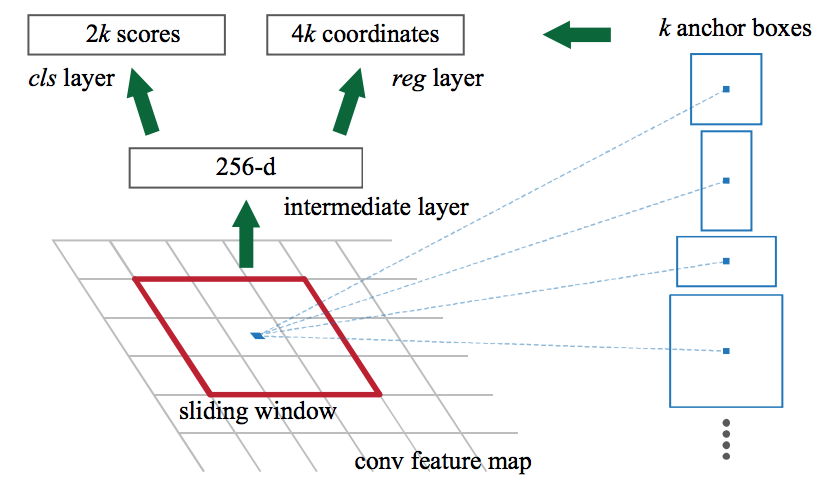
\includegraphics[width=\textwidth,height=8cm]{./Pictures/faster_rcnn_anchor.png}	
	\caption{Faster RCNN anchor示意图}	
	\label{anchor}
\end{uscfigure}

\textbf{3、位置精修和窗口分类:}分类层(cls\_score)计算每一个锚点上9个anchors属于前景和背景的概率;回归层(bbox\_pred)计算每一个锚点上9个anchors对应窗口平移缩放的参数。对于每个锚点输出$9*(4+1)$个参数












	\section{瓦片损害检测算法设计}
% 一些关于序号的设置
\setcounter{figure}{0}

\subsection{瓦片损害检测流程}
\subsection{SSD算法核心思想}
\subsection{SSD模型结构}
\subsection{SSD模型训练}
\subsection{算法改进方案}
\subsection{本章小结}
	\section{瓦片损害检测算法实现}
% 一些关于序号的设置
\setcounter{figure}{0}

\subsection{图像预处理}

	\section{实验结果与分析}
% 一些关于序号的设置
\setcounter{figure}{0}

\subsection{改进SSD算法的实验结果}
\begin{table}[htbp]
	\centering
	\caption{改进SSD算法的准确率实验结果}
	\label{}
	\begin{tabular}{ccc}
		\toprule
		网络模型 & mAP & fps\\
		\midrule
		SSD 	& 75\% & 60\\
		改进SSD  &  60\% & 50\\
		\bottomrule
	\end{tabular}
\end{table}
\subsection{改进SSD对瓦片损害检测的准确率实验}
\begin{table}[htbp]
	\centering
	\caption{改进SSD算法的准确率实验结果}
	\label{}
	\begin{tabular}{ccc}
		\toprule
		网络模型 & mAP & fps\\
		\midrule
		SSD 	& 75\% & 60\\
		改进SSD  &  60\% & 50\\
		\bottomrule
	\end{tabular}
\end{table}
\subsection{SSD 与修改了focus loss 的算法进行mAP、速度的比较}
\begin{table}[htbp]
	\centering
	\caption{改进SSD算法的准确率实验结果}
	\label{}
	\begin{tabular}{ccc}
		\toprule
		网络模型 & mAP & fps\\
		\midrule
		SSD 	& 75\% & 60\\
		改进SSD  &  60\% & 50\\
		\bottomrule
	\end{tabular}
\end{table}


	\section{总结及展望}
% 一些关于序号的设置
\setcounter{figure}{0}
\textbf{目标检测算法出现了以下几种:}

1、传统的目标检测算法:Cascade\cite{repid} + Haar\cite{haar} / SVM\cite{svm} + HOG / DPM ;

2、候选窗+深度学习分类:通过提取候选区域,并对相应区域进行以深度学习方法为主的分类的方案,如:RCNN / SPP-net/ Fast-RCNN / Faster-RCNN  / R-FCN\cite{rfcn}系列方法;

3、基于深度学习的回归方法:YOLO / SSD / DenseBox\cite{densebox}等方法;

4、结合RNN算法的RRC Detection;结合DPM的Deformable CNN\cite{deformable}等方法;

\textbf{基于深度学习方法的几个可能的方向:}

1、从原始图像、低层的Feature Map层,以及高层的语义层获取更多的信息,从而得到对目标Bounding Box的更准确的估计;

2、对Bounding Box的估计可以结合图片的一些由粗到细(coarse-to-fine)的分割信息;

3、对bounding box的估计需要引入更多的局部的content的信息;

4、目标检测数据集的标注难度非常大,如何把其他如classfication领域学习到的知识用于检测当中,甚至是将classification的数据和检测数据集做co-training(如YOLO9000)的方式,可以从数据层面获得更多的信息;

5、RRC,deformable cnn中卷积和其他的很好的图片的操作、机器学习的思想的结合未来也有很大的空间;

6、语意信息和分割的结合,可能能够为目标检测提供更多的有用的信息;

7、场景信息也会为目标检测提供更多信息;比如天空不会出现汽车等等。
	\bibliographystyle{unsrt}
	\bibliography{reference}
	\addcontentsline{toc}{section}{参考文献}	
	
	\section*{谢辞}
\addcontentsline{toc}{section}{谢辞}
白驹过隙,美好的大学生活匆匆而过,当毕业论文写到这章节的时候,满脑子的关于大学这四年的回忆,生命中有太多太多给予我帮助和陪伴我成长的人需要感谢。赋予我生命的爸爸妈妈给予我的关爱、计算机学院最负责任的老师——汪琳霞老师、308室友、物联网的同学们以及其它关心照顾我的人。在论文撰写之前我对深度学习相关知识还了解的不多,感谢刘立教授的悉心教导,以及对聚蜂智能科技有限公司的冉建大哥以及金华清同学的帮助表示感谢!
	\section*{附录}
\addcontentsline{toc}{section}{附录}
\subsection*{源代码}
\subsubsection*{datagen.py}
\begin{lstlisting}[caption={datagen.py}]
'''Load image/class/box from a annotation file.

The annotation file is organized as:
image_name #obj xmin ymin xmax ymax class_index ..
'''
from __future__ import print_function

import os
import sys
import os.path

import random
import numpy as np

import torch
import torch.utils.data as data
import torchvision.transforms as transforms

from encoder import DataEncoder
from PIL import Image, ImageOps


class ListDataset(data.Dataset):
img_size = 300

def __init__(self, root, list_file, train, transform):
'''
Args:
root: (str) ditectory to images.
list_file: (str) path to index file.
train: (boolean) train or test.
transform: ([transforms]) image transforms.
'''
self.root = root
self.train = train
self.transform = transform

self.fnames = []
self.boxes = []
self.labels = []

self.data_encoder = DataEncoder()

with open(list_file) as f:
lines = f.readlines()
self.num_samples = len(lines)

for line in lines:
splited = line.strip().split()
self.fnames.append(splited[0])

num_objs = int(splited[1])
box = []
label = []
for i in range(num_objs):
xmin = splited[2+5*i]
ymin = splited[3+5*i]
xmax = splited[4+5*i]
ymax = splited[5+5*i]
c = splited[6+5*i]
box.append([float(xmin),float(ymin),float(xmax),float(ymax)])
label.append(int(c))
self.boxes.append(torch.Tensor(box))
self.labels.append(torch.LongTensor(label))

def __getitem__(self, idx):
'''Load a image, and encode its bbox locations and class labels.

Args:
idx: (int) image index.

Returns:
img: (tensor) image tensor.
loc_target: (tensor) location targets, sized [8732,4].
conf_target: (tensor) label targets, sized [8732,].
'''
# Load image and bbox locations.
fname = self.fnames[idx]
img = Image.open(os.path.join(self.root, fname))
boxes = self.boxes[idx].clone()
labels = self.labels[idx]

# Data augmentation while training.
if self.train:
img, boxes = self.random_flip(img, boxes)
img, boxes, labels = self.random_crop(img, boxes, labels)

# Scale bbox locaitons to [0,1].
w,h = img.size
boxes /= torch.Tensor([w,h,w,h]).expand_as(boxes)

img = img.resize((self.img_size,self.img_size))
img = self.transform(img)

# Encode loc & conf targets.
loc_target, conf_target = self.data_encoder.encode(boxes, labels)
return img, loc_target, conf_target

def random_flip(self, img, boxes):
'''Randomly flip the image and adjust the bbox locations.

For bbox (xmin, ymin, xmax, ymax), the flipped bbox is:
(w-xmax, ymin, w-xmin, ymax).

Args:
img: (PIL.Image) image.
boxes: (tensor) bbox locations, sized [#obj, 4].

Returns:
img: (PIL.Image) randomly flipped image.
boxes: (tensor) randomly flipped bbox locations, sized [#obj, 4].
'''
if random.random() < 0.5:
img = img.transpose(Image.FLIP_LEFT_RIGHT)
w = img.width
xmin = w - boxes[:,2]
xmax = w - boxes[:,0]
boxes[:,0] = xmin
boxes[:,2] = xmax
return img, boxes

def random_crop(self, img, boxes, labels):
'''Randomly crop the image and adjust the bbox locations.

For more details, see 'Chapter2.2: Data augmentation' of the paper.

Args:
img: (PIL.Image) image.
boxes: (tensor) bbox locations, sized [#obj, 4].
labels: (tensor) bbox labels, sized [#obj,].

Returns:
img: (PIL.Image) cropped image.
selected_boxes: (tensor) selected bbox locations.
labels: (tensor) selected bbox labels.
'''
imw, imh = img.size
while True:
min_iou = random.choice([None, 0.1, 0.3, 0.5, 0.7, 0.9])
if min_iou is None:
return img, boxes, labels

for _ in range(100):
w = random.randrange(int(0.1*imw), imw)
h = random.randrange(int(0.1*imh), imh)

if h > 2*w or w > 2*h:
continue

x = random.randrange(imw - w)
y = random.randrange(imh - h)
roi = torch.Tensor([[x, y, x+w, y+h]])

center = (boxes[:,:2] + boxes[:,2:]) / 2  # [N,2]
roi2 = roi.expand(len(center), 4)  # [N,4]
mask = (center > roi2[:,:2]) & (center < roi2[:,2:])  # [N,2]
mask = mask[:,0] & mask[:,1]  #[N,]
if not mask.any():
continue

selected_boxes = boxes.index_select(0, mask.nonzero().squeeze(1))

iou = self.data_encoder.iou(selected_boxes, roi)
if iou.min() < min_iou:
continue

img = img.crop((x, y, x+w, y+h))
selected_boxes[:,0].add_(-x).clamp_(min=0, max=w)
selected_boxes[:,1].add_(-y).clamp_(min=0, max=h)
selected_boxes[:,2].add_(-x).clamp_(min=0, max=w)
selected_boxes[:,3].add_(-y).clamp_(min=0, max=h)
return img, selected_boxes, labels[mask]

def __len__(self):
return self.num_samples
\end{lstlisting}
\subsubsection*{ssd.py}
\begin{lstlisting}
import math
import itertools

import torch
import torch.nn as nn
import torch.nn.functional as F
import torch.nn.init as init

from torch.autograd import Variable

from multibox_layer import MultiBoxLayer


class L2Norm2d(nn.Module):
'''L2Norm layer across all channels.'''
def __init__(self, scale):
super(L2Norm2d, self).__init__()
self.scale = scale

def forward(self, x, dim=1):
'''out = scale * x / sqrt(\sum x_i^2)'''
return self.scale * x * x.pow(2).sum(dim).clamp(min=1e-12).
	rsqrt().expand_as(x)


class SSD300(nn.Module):
input_size = 300

def __init__(self):
super(SSD300, self).__init__()

# model
self.base = self.VGG16()
self.norm4 = L2Norm2d(20)

self.conv5_1 = nn.Conv2d(512, 512, kernel_size=3, padding=1, dilation=1)
self.conv5_2 = nn.Conv2d(512, 512, kernel_size=3, padding=1, dilation=1)
self.conv5_3 = nn.Conv2d(512, 512, kernel_size=3, padding=1, dilation=1)

self.conv6 = nn.Conv2d(512, 1024, kernel_size=3, padding=6, dilation=6)

self.conv7 = nn.Conv2d(1024, 1024, kernel_size=1)

self.conv8_1 = nn.Conv2d(1024, 256, kernel_size=1)
self.conv8_2 = nn.Conv2d(256, 512, kernel_size=3, padding=1, stride=2)

self.conv9_1 = nn.Conv2d(512, 128, kernel_size=1)
self.conv9_2 = nn.Conv2d(128, 256, kernel_size=3, padding=1, stride=2)

self.conv10_1 = nn.Conv2d(256, 128, kernel_size=1)
self.conv10_2 = nn.Conv2d(128, 256, kernel_size=3)

self.conv11_1 = nn.Conv2d(256, 128, kernel_size=1)
self.conv11_2 = nn.Conv2d(128, 256, kernel_size=3)

# multibox layer
self.multibox = MultiBoxLayer()

def forward(self, x):
hs = []
h = self.base(x)
hs.append(self.norm4(h))  # conv4_3

h = F.max_pool2d(h, kernel_size=2, stride=2, ceil_mode=True)

h = F.relu(self.conv5_1(h))
h = F.relu(self.conv5_2(h))
h = F.relu(self.conv5_3(h))
h = F.max_pool2d(h, kernel_size=3, padding=1, stride=1, ceil_mode=True)

h = F.relu(self.conv6(h))
h = F.relu(self.conv7(h))
hs.append(h)  # conv7

h = F.relu(self.conv8_1(h))
h = F.relu(self.conv8_2(h))
hs.append(h)  # conv8_2

h = F.relu(self.conv9_1(h))
h = F.relu(self.conv9_2(h))
hs.append(h)  # conv9_2

h = F.relu(self.conv10_1(h))
h = F.relu(self.conv10_2(h))
hs.append(h)  # conv10_2

h = F.relu(self.conv11_1(h))
h = F.relu(self.conv11_2(h))
hs.append(h)  # conv11_2

loc_preds, conf_preds = self.multibox(hs)
return loc_preds, conf_preds

def VGG16(self):
'''VGG16 layers.'''
cfg = [64, 64, 'M', 128, 128, 'M', 256, 256, 256, 'M', 512, 512, 512]
layers = []
in_channels = 3
for x in cfg:
if x == 'M':
layers += [nn.MaxPool2d(kernel_size=2, stride=2, ceil_mode=True)]
else:
layers += [nn.Conv2d(in_channels, x, kernel_size=3, padding=1),
nn.ReLU(True)]
in_channels = x
return nn.Sequential(*layers)
\end{lstlisting}

\subsubsection*{multibox\_layer.py}
\begin{lstlisting}
from __future__ import print_function

import math

import torch
import torch.nn as nn
import torch.nn.init as init
import torch.nn.functional as F

from torch.autograd import Variable


class MultiBoxLayer(nn.Module):
num_classes = 21
num_anchors = [4,6,6,6,4,4]
in_planes = [512,1024,512,256,256,256]

def __init__(self):
super(MultiBoxLayer, self).__init__()

self.loc_layers = nn.ModuleList()
self.conf_layers = nn.ModuleList()
for i in range(len(self.in_planes)):
self.loc_layers.append(nn.Conv2d(self.in_planes[i],
 self.num_anchors[i]*4, kernel_size=3, padding=1))
self.conf_layers.append(nn.Conv2d(self.in_planes[i],
 self.num_anchors[i]*21, kernel_size=3, padding=1))

def forward(self, xs):
'''
Args:
xs: (list) of tensor containing intermediate layer outputs.

Returns:
loc_preds: (tensor) predicted locations, sized [N,8732,4].
conf_preds: (tensor) predicted class confidences,
 sized [N,8732,21].
'''
y_locs = []
y_confs = []
for i,x in enumerate(xs):
y_loc = self.loc_layers[i](x)
N = y_loc.size(0)
y_loc = y_loc.permute(0,2,3,1).contiguous()
y_loc = y_loc.view(N,-1,4)
y_locs.append(y_loc)

y_conf = self.conf_layers[i](x)
y_conf = y_conf.permute(0,2,3,1).contiguous()
y_conf = y_conf.view(N,-1,21)
y_confs.append(y_conf)

loc_preds = torch.cat(y_locs, 1)
conf_preds = torch.cat(y_confs, 1)
return loc_preds, conf_preds
\end{lstlisting}

\subsubsection*{multibox\_loss.py}
\begin{lstlisting}
from __future__ import print_function

import math

import torch
import torch.nn as nn
import torch.nn.init as init
import torch.nn.functional as F

from torch.autograd import Variable


class MultiBoxLoss(nn.Module):
num_classes = 21

def __init__(self):
super(MultiBoxLoss, self).__init__()

def cross_entropy_loss(self, x, y):
'''Cross entropy loss w/o averaging across all samples.

Args:
x: (tensor) sized [N,D].
y: (tensor) sized [N,].

Return:
(tensor) cross entroy loss, sized [N,].
'''
xmax = x.data.max()
log_sum_exp = torch.log(torch.sum(torch.exp(x-xmax), 1)) + xmax
return log_sum_exp - x.gather(1, y.view(-1,1))

def test_cross_entropy_loss(self):
a = Variable(torch.randn(10,4))
b = Variable(torch.ones(10).long())
loss = self.cross_entropy_loss(a,b)
print(loss.mean())
print(F.cross_entropy(a,b))

def hard_negative_mining(self, conf_loss, pos):
'''Return negative indices that is 3x the 
number as postive indices.

Args:
conf_loss: (tensor) cross entroy loss 
between conf_preds and conf_targets, sized [N*8732,].
pos: (tensor) positive(matched) box indices, sized [N,8732].

Return:
(tensor) negative indices, sized [N,8732].
'''
batch_size, num_boxes = pos.size()

conf_loss[pos] = 0  # set pos boxes = 0, 
the rest are neg conf_loss
conf_loss = conf_loss.view(batch_size, -1)  # [N,8732]

_,idx = conf_loss.sort(1, descending=True)  # sort by neg conf_loss
_,rank = idx.sort(1)  # [N,8732]

num_pos = pos.long().sum(1)  # [N,1]
num_neg = torch.clamp(3*num_pos, max=num_boxes-1)  # [N,1]

neg = rank < num_neg.expand_as(rank)  # [N,8732]
return neg

def forward(self, loc_preds, loc_targets, conf_preds, conf_targets):
'''Compute loss between (loc_preds, loc_targets) and (conf_preds, conf_targets).

Args:
loc_preds: (tensor) predicted locations, sized [batch_size, 8732, 4].
loc_targets: (tensor) encoded target locations, sized [batch_size, 8732, 4].
conf_preds: (tensor) predicted class confidences, sized [batch_size, 8732, num_classes].
conf_targets: (tensor) encoded target classes, sized [batch_size, 8732].

loss:
(tensor) loss = SmoothL1Loss(loc_preds, loc_targets) + CrossEntropyLoss(conf_preds, conf_targets).
'''
batch_size, num_boxes, _ = loc_preds.size()

pos = conf_targets>0  # [N,8732], pos means the box matched.
num_matched_boxes = pos.data.long().sum()
if num_matched_boxes == 0:
return Variable(torch.Tensor([0]))

################################################################
# loc_loss = SmoothL1Loss(pos_loc_preds, pos_loc_targets)
################################################################
pos_mask = pos.unsqueeze(2).expand_as(loc_preds)    # [N,8732,4]
pos_loc_preds = loc_preds[pos_mask].view(-1,4)      # [#pos,4]
pos_loc_targets = loc_targets[pos_mask].view(-1,4)  # [#pos,4]
loc_loss = F.smooth_l1_loss(pos_loc_preds, pos_loc_targets, size_average=False)

################################################################
# conf_loss = CrossEntropyLoss(pos_conf_preds, pos_conf_targets)
#           + CrossEntropyLoss(neg_conf_preds, neg_conf_targets)
################################################################
conf_loss = self.cross_entropy_loss(conf_preds.view(
-1,self.num_classes), 
conf_targets.view(-1))  # [N*8732,]
neg = self.hard_negative_mining(conf_loss, pos)    # [N,8732]

pos_mask = pos.unsqueeze(2).expand_as(conf_preds)  # [N,8732,21]
neg_mask = neg.unsqueeze(2).expand_as(conf_preds)  # [N,8732,21]
mask = (pos_mask+neg_mask).gt(0)

pos_and_neg = (pos+neg).gt(0)
preds = conf_preds[mask].view(-1,self.num_classes)  # [#pos+#neg,21]
targets = conf_targets[pos_and_neg]                 # [#pos+#neg,]
conf_loss = F.cross_entropy(preds, targets, size_average=False)

loc_loss /= num_matched_boxes
conf_loss /= num_matched_boxes
print('%f %f' % (loc_loss.data[0], conf_loss.data[0]), end=' ')
return loc_loss + conf_loss
\end{lstlisting}
\subsubsection*{encoder.py}
\begin{lstlisting}
'''Encode target locations and labels.'''
import torch

import math
import itertools

class DataEncoder:
def __init__(self):
'''Compute default box sizes with scale and aspect transform.'''
scale = 300.
steps = [s / scale for s in (8, 16, 32, 64, 100, 300)]
sizes = [s / scale for s in (30, 60, 111, 162, 213, 264, 315)]
aspect_ratios = ((2,), (2,3), (2,3), (2,3), (2,), (2,))
feature_map_sizes = (38, 19, 10, 5, 3, 1)

num_layers = len(feature_map_sizes)

boxes = []
for i in range(num_layers):
fmsize = feature_map_sizes[i]
for h,w in itertools.product(range(fmsize), repeat=2):
cx = (w + 0.5)*steps[i]
cy = (h + 0.5)*steps[i]

s = sizes[i]
boxes.append((cx, cy, s, s))

s = math.sqrt(sizes[i] * sizes[i+1])
boxes.append((cx, cy, s, s))

s = sizes[i]
for ar in aspect_ratios[i]:
boxes.append((cx, cy, s * math.sqrt(ar), s / math.sqrt(ar)))
boxes.append((cx, cy, s / math.sqrt(ar), s * math.sqrt(ar)))

self.default_boxes = torch.Tensor(boxes)

def iou(self, box1, box2):
'''Compute the intersection over union of 
two set of boxes, each box is [x1,y1,x2,y2].

Args:
box1: (tensor) bounding boxes, sized [N,4].
box2: (tensor) bounding boxes, sized [M,4].

Return:
(tensor) iou, sized [N,M].
'''
N = box1.size(0)
M = box2.size(0)

lt = torch.max(
box1[:,:2].unsqueeze(1).expand(N,M,2),  # [N,2] -> [N,1,2] -> [N,M,2]
box2[:,:2].unsqueeze(0).expand(N,M,2),  # [M,2] -> [1,M,2] -> [N,M,2]
)

rb = torch.min(
box1[:,2:].unsqueeze(1).expand(N,M,2),  # [N,2] -> [N,1,2] -> [N,M,2]
box2[:,2:].unsqueeze(0).expand(N,M,2),  # [M,2] -> [1,M,2] -> [N,M,2]
)

wh = rb - lt  # [N,M,2]
wh[wh<0] = 0  # clip at 0
inter = wh[:,:,0] * wh[:,:,1]  # [N,M]

area1 = (box1[:,2]-box1[:,0]) * (box1[:,3]-box1[:,1])  # [N,]
area2 = (box2[:,2]-box2[:,0]) * (box2[:,3]-box2[:,1])  # [M,]
area1 = area1.unsqueeze(1).expand_as(inter)  # [N,] -> [N,1] -> [N,M]
area2 = area2.unsqueeze(0).expand_as(inter)  # [M,] -> [1,M] -> [N,M]

iou = inter / (area1 + area2 - inter)
return iou

def encode(self, boxes, classes, threshold=0.5):
'''Transform target bounding boxes and class labels 
to SSD boxes and classes.

Match each object box to all the default boxes, pick 
the ones with the
Jaccard-Index > 0.5:
Jaccard(A,B) = AB / (A+B-AB)

Args:
boxes: (tensor) object bounding boxes
 (xmin,ymin,xmax,ymax) of a image, sized [#obj, 4].
classes: (tensor) object class labels of a image, sized [#obj,].
threshold: (float) Jaccard index threshold

Returns:
boxes: (tensor) bounding boxes, sized [#obj, 8732, 4].
classes: (tensor) class labels, sized [8732,]
'''
default_boxes = self.default_boxes
num_default_boxes = default_boxes.size(0)
num_objs = boxes.size(0)

iou = self.iou(  # [#obj,8732]
boxes,
torch.cat([default_boxes[:,:2] - default_boxes[:,2:]/2,
default_boxes[:,:2] + default_boxes[:,2:]/2], 1)
)

iou, max_idx = iou.max(0)  # [1,8732]
max_idx.squeeze_(0)        # [8732,]
iou.squeeze_(0)            # [8732,]

boxes = boxes[max_idx]     # [8732,4]
variances = [0.1, 0.2]
cxcy = (boxes[:,:2] + boxes[:,2:])/2 - default_boxes[:,:2]  # [8732,2]
cxcy /= variances[0] * default_boxes[:,2:]
wh = (boxes[:,2:] - boxes[:,:2]) / default_boxes[:,2:]      # [8732,2]
wh = torch.log(wh) / variances[1]
loc = torch.cat([cxcy, wh], 1)  # [8732,4]

conf = 1 + classes[max_idx]   # [8732,], background class = 0
conf[iou<threshold] = 0       # background
return loc, conf

def nms(self, bboxes, scores, threshold=0.5, mode='union'):
'''Non maximum suppression.

Args:
bboxes: (tensor) bounding boxes, sized [N,4].
scores: (tensor) bbox scores, sized [N,].
threshold: (float) overlap threshold.
mode: (str) 'union' or 'min'.

Returns:
keep: (tensor) selected indices.

Ref:
https://github.com/rbgirshick/py-faster-rcnn/
blob/master/lib/nms/py_cpu_nms.py
'''
x1 = bboxes[:,0]
y1 = bboxes[:,1]
x2 = bboxes[:,2]
y2 = bboxes[:,3]

areas = (x2-x1) * (y2-y1)
_, order = scores.sort(0, descending=True)

keep = []
while order.numel() > 0:
i = order[0]
keep.append(i)

if order.numel() == 1:
break

xx1 = x1[order[1:]].clamp(min=x1[i])
yy1 = y1[order[1:]].clamp(min=y1[i])
xx2 = x2[order[1:]].clamp(max=x2[i])
yy2 = y2[order[1:]].clamp(max=y2[i])

w = (xx2-xx1).clamp(min=0)
h = (yy2-yy1).clamp(min=0)
inter = w*h

if mode == 'union':
ovr = inter / (areas[i] + areas[order[1:]] - inter)
elif mode == 'min':
ovr = inter / areas[order[1:]].clamp(max=areas[i])
else:
raise TypeError('Unknown nms mode: %s.' % mode)

ids = (ovr<=threshold).nonzero().squeeze()
if ids.numel() == 0:
break
order = order[ids+1]
return torch.LongTensor(keep)

def decode(self, loc, conf):
'''Transform predicted loc/conf back to real bbox
 locations and class labels.

Args:
loc: (tensor) predicted loc, sized [8732,4].
conf: (tensor) predicted conf, sized [8732,21].

Returns:
boxes: (tensor) bbox locations, sized [#obj, 4].
labels: (tensor) class labels, sized [#obj,1].
'''
variances = [0.1, 0.2]
wh = torch.exp(loc[:,2:]*variances[1]) * self.default_boxes[:,2:]
cxcy = loc[:,:2] * variances[0] *
 self.default_boxes[:,2:] + self.default_boxes[:,:2]
boxes = torch.cat([cxcy-wh/2, cxcy+wh/2], 1)  # [8732,4]

max_conf, labels = conf.max(1)  # [8732,1]
ids = labels.squeeze(1).nonzero().squeeze(1)  # [#boxes,]

keep = self.nms(boxes[ids], max_conf[ids].squeeze(1))
return boxes[ids][keep], labels[ids][keep], max_conf[ids][keep]
\end{lstlisting}

\end{document}